\documentclass[10pt, aspectratio=169]{beamer}
\usefonttheme{professionalfonts}

\mode<presentation>
{
  \usetheme{Berkeley}
  \usecolortheme{beaver}
  \usefonttheme{default}
  \setbeamertemplate{navigation symbols}{}
  \setbeamertemplate{caption}[numbered]
} 

\setbeamertemplate{footline}{%
  \leavevmode%
  \hbox{%
    \begin{beamercolorbox}[wd=.85\paperwidth,ht=2.5ex,dp=1ex,left]{author in head/foot}%
      \usebeamerfont{author in head/foot}Maxx Seminario, Electronic Circuits, Fall 2025%
    \end{beamercolorbox}%
    \begin{beamercolorbox}[wd=.15\paperwidth,ht=2.5ex,dp=1ex,right]{date in head/foot}%
      \hspace*{0.5em}\insertframenumber{} / \inserttotalframenumber\hspace*{0.5em}%
    \end{beamercolorbox}%
  }%
  \vskip0pt%
}

\usepackage[english]{babel}
\usepackage[utf8x]{inputenc}
\usepackage{tikz}
\usetikzlibrary{shapes.geometric}
\usepackage{pgfplots}
\usepackage{array}
\usepackage{makecell}
\usepackage{verbatim}
\usepackage{graphicx}
\usepackage{subcaption}
\usepackage{amsfonts}
\usepackage{amsmath}
\usepackage{bm}
\usepackage{epstopdf}
\usepackage{circuitikz}
\usepackage{caption}
\captionsetup{compatibility=false}
\usepackage[absolute,overlay]{textpos}
\usetikzlibrary{calc}
\usetikzlibrary{pgfplots.fillbetween, backgrounds}
\usetikzlibrary{fit}
\usetikzlibrary{positioning}
\usetikzlibrary{pgfplots.groupplots}
\usetikzlibrary{plotmarks}
\usetikzlibrary{calc}
\usepgfplotslibrary{groupplots}
\pgfplotsset{compat=newest} 

% Added by Maxx Seminario 01/06/2026 - for colored icons in itemize labels
\usepackage{wasysym} % for smiles and frowns
\newcommand{\neutralface}{%
  \tikz[baseline=-0.6ex]{
    \draw (0,0) circle (0.9ex);
    \fill (-0.35ex,0.25ex) circle (0.12ex);
    \fill ( 0.35ex,0.25ex) circle (0.12ex);
    \draw (-0.35ex,-0.25ex) -- (0.35ex,-0.25ex);
  }%
}

\newcommand{\baditem}{\textcolor{red!70!black}{\frownie}}
\newcommand{\gooditem}{\textcolor{green!60!black}{\smiley}}
\newcommand{\mehitem}{\textcolor{orange!80!black}{\neutralface}}


\usepackage{hyperref}
\definecolor{BeaverRed}{RGB}{179,38,38} 
\hypersetup{
    colorlinks=true,
    linkcolor=BeaverRed,
    filecolor=magenta,      
    urlcolor=cyan,
}

% =========================
% Solution toggle 
% =========================
\newif\ifshowsolutions
\showsolutionstrue   %  compile WITH solutions
%\showsolutionsfalse %  compile WITHOUT solutions

% =========================
% Document Information
% =========================
\title[Op-Amp Applications]{Operational Amplifier Applications}
\subtitle{Feedback Configurations and Mathematical Operations}
\author{Maxx Seminario}
\institute{University of Nebraska-Lincoln}
\date{Spring 2026}

\begin{document}

\begin{frame}
  \titlepage
\end{frame}

\begin{frame}{Outline}
  \tableofcontents
\end{frame}

\section{Review and Negative Feedback}

\begin{frame}{Review:  The Ideal Op-Amp}
    
    \begin{columns}[t]
    \column{0.48\textwidth}
        \textbf{Five Ideal OpAmp Assumptions}: 
        \begin{enumerate}
            \item $Z_{in} = \infty$ $\Rightarrow$ $i_+ = i_- = 0$
            \item $Z_{out} = 0$ (ideal voltage source)
            \item $A = \infty$ (infinite open-loop gain)
            \item Infinite bandwidth
            \item Infinite CMRR
        \end{enumerate}
        
        \vspace{0.3cm}
        
        \textbf{Basic Relationship}:
        \[
        v_{out} = A(v_+ - v_-)
        \]
        
        With $A \to \infty$, for bounded output:
        \[
        v_+ - v_- \to 0 \quad \text{(virtual short)}
        \]
        
    \column{0.48\textwidth}
        \begin{figure}[t]
        \centering
        \begin{circuitikz}[scale=0.7]
            % Op-amp
            \draw (0,0) node[op amp, yscale=1.5] (opamp) {};
            
            % Labels
            \node at (opamp.-) [left, xshift=-0.3cm] {$v_-$};
            \node at (opamp.+) [left, xshift=-0.3cm] {$v_+$};
            \node at (opamp.out) [right, xshift=0.3cm] {$v_{out}$};
            
            % Current annotations
            \draw[->, red, thick] (opamp.- |- 0,0.8) -- ++(0,0.5) node[above] {$i_-=0$};
            \draw[->, red, thick] (opamp.+ |- 0,-0.8) -- ++(0,-0.5) node[below] {$i_+=0$};
            
        \end{circuitikz}
        \caption{Ideal op-amp terminals}
        \end{figure}
        
        \begin{block}{Key Insight}
            \begin{itemize}
                \item $v_+ = v_-$ (virtual short)
                \item $i_+ = i_- = 0$ (no input current)
            \end{itemize}
        \end{block}
        
    \end{columns}
    
\end{frame}

\begin{frame}{Negative Feedback Concept}
    
    \begin{columns}[t]
    \column{0.48\textwidth}
        \textbf{What is Negative Feedback?}
        \begin{itemize}
            \item Output is fed back to inverting input
            \item Opposes changes in output
            \item[\gooditem] Makes gain predictable
        \end{itemize}
        
        \textbf{Why Use Feedback?}
        \begin{itemize}
            \item[\gooditem] Precise, stable gain
            \item[\gooditem] Insensitive to $A$ variations
            \item[\gooditem] Improved linearity
            \item[\gooditem] Controlled impedances
        \end{itemize}
        
        \begin{alertblock}{Key Insight}
            With negative feedback and ideal op-amp:  $v_+ = v_-$
        \end{alertblock}
        
    \column{0.48\textwidth}
    \begin{figure}[htb]
    \centering
    \begin{circuitikz}[
        scale=0.75,
        every node/.style={font=\small}
    ]
        % Input wire
        \draw (0,0) node[left] {$v_{in}$} to[short, o-] (1.2,0);

        % Op-amp 
        \node[op amp, scale=0.9] (opamp) at (2.6,0) {};

        % Connect input to + input
        \draw (1.2,0) -- (opamp.+);

        % Output
        \draw (opamp.out) to[short, -o] (4.6,0) node[right] {$v_{out}$};

        % Feedback 
        \coordinate (fbup) at ($(opamp.out)+(0,1.8)$);
        \draw (opamp.out) -- (fbup);
        \draw[red, thick, ->] (fbup) -| (opamp.-)
            node[pos=0.25, above] {feedback};

        % Blue block neatly around the op-amp using fit
        \node[
            draw,
            blue,
            thick,
            rounded corners,
            inner sep=6pt,
            fit=(opamp)
        ] (ampblock) {};

        % Optional label centered under the block
        \node[blue] at ($(ampblock.south)+(0,-0.35)$) {Amplifier};

    \end{circuitikz}
    \caption{Negative feedback block diagram}
    \end{figure}


        \textbf{Result}:
        \begin{itemize}
            \item Op-amp adjusts $v_{out}$ to make $v_- = v_+$
            \item[\gooditem] Gain determined by external components
            \item[\gooditem] Not by internal gain $A$
        \end{itemize}
        
    \end{columns}
    
\end{frame}

\section{Inverting Amplifier}

\begin{frame}{The Inverting Amplifier}
    
    \begin{columns}[t]
    \column{0.48\textwidth}
        \textbf{Circuit Configuration}: 
        
    \begin{figure}[htb]
    \centering
    \begin{circuitikz}[scale=0.8, every node/.style={font=\small}]
        % Op-amp
        \node[op amp, scale=1.0] (opamp) at (3,0) {};

        % Left input point aligned horizontally with the inverting input
        \coordinate (vin) at ($(opamp.-)+(-3.0,0)$);

        % Input resistor (perfectly horizontal)
        \draw (vin) node[left] {$v_{in}$}
            to[R, l=$R_1$, o-] (opamp.-);

        % Non-inverting input to ground
        \draw (opamp.+) -- ++(0,-1.0) node[ground] {};

        % Output
        \draw (opamp.out) to[short, -o] (5.2,0) node[right] {$v_{out}$};

        % Feedback resistor from output back to inverting input
        \draw (opamp.out) -- ++(0,1.6)
            to[R, l=$R_f$] ++(-3.0,0)
            |- (opamp.-);

    \end{circuitikz}
    \caption{Inverting amplifier circuit}
    \end{figure}

    \column{0.48\textwidth}
        \textbf{Analysis}:
        
        1. Since $v_+ = 0$ (AC Ground, be careful!):
        \[
        v_- = v_+ = 0 \quad \text{(AC ground)}
        \]
        
        2. Current through $R_1$:
        \[
        i_1 = \frac{v_{in} - v_-}{R_1} = \frac{v_{in}}{R_1}
        \]
        
        3. Since $i_- = 0$, all of $i_1$ flows through $R_f$:
        \[
        i_f = i_1 = \frac{v_{in}}{R_1}
        \]
        
        4. Voltage across $R_f$:
        \[
        v_{out} - v_- = -i_f R_f
        \]
        \[
        v_{out} = -i_f R_f = -\frac{R_f}{R_1} v_{in}
        \]
        
    \end{columns}
    
\end{frame}

\begin{frame}{Inverting Amplifier:  Results}
    
    \begin{columns}[t]
    \column{0.48\textwidth}
        \textbf{Voltage Gain}:
        \[
        \boxed{A_v = \frac{v_{out}}{v_{in}} = -\frac{R_f}{R_1}}
        \]
        
        \begin{itemize}
            \item[\mehitem] Negative sign:  180° phase shift
            \item[\gooditem] Magnitude set by resistor ratio
            \item[\gooditem] Independent of op-amp gain $A$
        \end{itemize}
        
        \textbf{Input Impedance}:
        \[
        \boxed{R_{in} = \frac{v_{in}}{i_1} = R_1}
        \]
        
        \begin{itemize}
            \item[\mehitem] Not infinite! 
            \item[\gooditem] Determined by $R_1$
        \end{itemize}
        
    \column{0.48\textwidth}
        \textbf{Design Examples}:

        
        \textbf{Example 1}: Unity gain inverter
        \begin{itemize}
            \item $R_1 = R_f = 10$ k$\Omega$
            \item $A_v = -1$
            \item $R_{in} = 10$ k$\Omega$
        \end{itemize}

        \textbf{Example 2}: Gain of -10
        \begin{itemize}
            \item $R_1 = 10$ k$\Omega$, $R_f = 100$ k$\Omega$
            \item $A_v = -10$
            \item $R_{in} = 10$ k$\Omega$
        \end{itemize}

        \textbf{Example 3}: Gain of -0.5
        \begin{itemize}
            \item $R_1 = 20$ k$\Omega$, $R_f = 10$ k$\Omega$
            \item $A_v = -0.5$ (attenuation!)
            \item $R_{in} = 20$ k$\Omega$
        \end{itemize}
        
    \end{columns}
    
\end{frame}

\section{Noninverting Amplifier}

\begin{frame}{The Noninverting Amplifier}
    
    \begin{columns}[t]
    \column{0.48\textwidth}
        \textbf{Circuit Configuration}:
        
        \begin{figure}[htb]
        \centering
        \begin{circuitikz}[scale=1.0]
            % Input to noninverting terminal
            \draw (0,0) to[short, o-] (1,0);
            
            % Op-amp
            \draw (2.5,-0.5) node[op amp, yscale=1.3] (opamp) {};
            
            % Input connection
            \draw (1,0) |- (opamp.+);
            
            % Ground reference
            \draw (1,0) to[short, *-] (1,-1) node[ground] {};
            
            % Feedback network
            \draw (opamp.-) -- ++(0,1.5) coordinate(fb1);
            \draw (fb1) to[R, l=$R_f$] (fb1 -| opamp.out);
            \draw (opamp.out) |- (fb1 -| opamp.out);
            
            % Bottom resistor to ground
            \draw (opamp.-) to[R, l_=$R_1$] (opamp.- |- 0,-2) node[ground] {};
            
            % Output
            \draw (opamp.out) to[short, -o] (5,-0.5) node[right] {$v_{out}$};
            
            % Labels
            \node[left] at (0,0) {$v_{in}$};
            \node at (opamp.-) [left, xshift=-0.2cm] {$v_-$};
            
        \end{circuitikz}
        \caption{Noninverting amplifier circuit}
        \end{figure}
        
    \column{0.48\textwidth}
        \textbf{Analysis}:
        
        1. Since $v_+ = v_{in}$:
        \[
        v_- = v_+ = v_{in}
        \]
        
        2. Voltage divider at inverting input:
        \[
        v_- = v_{out} \frac{R_1}{R_1 + R_f}
        \]
        
        3. Equating the two expressions:
        \[
        v_{in} = v_{out} \frac{R_1}{R_1 + R_f}
        \]
        
        4. Solving for gain:
        \[
        \frac{v_{out}}{v_{in}} = \frac{R_1 + R_f}{R_1}
        \]
        \[
        \boxed{A_v = 1 + \frac{R_f}{R_1}}
        \]
        
    \end{columns}
    
\end{frame}

\begin{frame}{Noninverting Amplifier: Key Results}
    
    \begin{columns}[t]
    \column{0.48\textwidth}
        \textbf{Voltage Gain}:
        \[
        \boxed{A_v = 1 + \frac{R_f}{R_1}}
        \]
        
        \begin{itemize}
            \item Always positive (no inversion)
            \item Minimum gain is 1
            \item Set by resistor ratio
        \end{itemize}
        
        \vspace{0.3cm}
        
        \textbf{Input Impedance}: 
        \[
        \boxed{R_{in} = \infty}
        \]
        
        \begin{itemize}
            \item Infinite (ideally)
            \item Input goes to op-amp $+$ terminal
            \item No loading of source
        \end{itemize}
        
        \vspace{0.3cm}
        
        \textbf{Special Case - Voltage Follower}:
        \begin{itemize}
            \item $R_f = 0$ (short circuit)
            \item $R_1 = \infty$ (open circuit)
            \item $A_v = 1$ (unity gain buffer)
        \end{itemize}
        
    \column{0.48\textwidth}
        \textbf{Design Examples}:
        
        \vspace{0.2cm}
        
        \textbf{Example 1}:  Gain of 2
        \begin{itemize}
            \item $R_1 = R_f = 10$ k$\Omega$
            \item $A_v = 1 + 1 = 2$
        \end{itemize}
        
        \vspace{0.2cm}
        
        \textbf{Example 2}:  Gain of 11
        \begin{itemize}
            \item $R_1 = 10$ k$\Omega$, $R_f = 100$ k$\Omega$
            \item $A_v = 1 + 10 = 11$
        \end{itemize}
        
        \vspace{0.2cm}
        
        \textbf{Voltage Follower}:
        
        \begin{figure}[htb]
        \centering
        \begin{circuitikz}[scale=0.8]
            % Input
            \draw (0,0) to[short, o-] (1,0);
            
            % Op-amp
            \draw (2,-0.5) node[op amp, yscale=1.2] (opamp) {};
            \draw (1,0) |- (opamp.+);
            
            % Direct feedback
            \draw (opamp.out) |- ++(0,0.8) -| (opamp.-);
            
            % Output
            \draw (opamp.out) to[short, -o] (4,-0.5) node[right] {$v_{out}$};
            
            % Labels
            \node[left] at (0,0) {$v_{in}$};
        \end{circuitikz}
        \caption{Unity gain buffer ($A_v = 1$)}
        \end{figure}
        
    \end{columns}
    
\end{frame}

\section{Summing Amplifier}

\begin{frame}{The Summing Amplifier}
    
    \begin{columns}[t]
    \column{0.48\textwidth}
        \textbf{Circuit Configuration}:
        
        \begin{figure}[htb]
        \centering
        \begin{circuitikz}[scale=0.9]
            % Multiple inputs
            \draw (0,1.5) to[R, l=$R_1$, o-] (2,1.5);
            \draw (0,0.5) to[R, l=$R_2$, o-] (2,0.5);
            \draw (0,-0.5) to[R, l=$R_3$, o-] (2,-0.5);
            
            % Junction at inverting input
            \draw (2,1.5) -- (2,0);
            \draw (2,0.5) -- (2,0);
            \draw (2,-0.5) -- (2,0);
            
            % Op-amp
            \draw (3,-0.5) node[op amp, yscale=1.3] (opamp) {};
            \draw (2,0) |- (opamp.-);
            
            % Ground to noninverting
            \draw (opamp.+) -- ++(0,-0.5) node[ground] {};
            
            % Feedback resistor
            \draw (opamp.-) -- ++(0,1.5) coordinate(fb1);
            \draw (fb1) to[R, l=$R_f$] (fb1 -| opamp.out);
            \draw (opamp.out) |- (fb1 -| opamp.out);
            
            % Output
            \draw (opamp.out) to[short, -o] (5.5,-0.5) node[right] {$v_{out}$};
            
            % Input labels
            \node[left] at (0,1.5) {$v_1$};
            \node[left] at (0,0.5) {$v_2$};
            \node[left] at (0,-0.5) {$v_3$};
            \node at (2,0) [above] {$v_-=0$};
            
        \end{circuitikz}
        \caption{Summing amplifier (3 inputs)}
        \end{figure}
        
    \column{0.48\textwidth}
        \textbf{Analysis}:
        
        1. Virtual ground:  $v_- = 0$
        
        2. Currents from each input:
        \[
        i_1 = \frac{v_1}{R_1}, \quad i_2 = \frac{v_2}{R_2}, \quad i_3 = \frac{v_3}{R_3}
        \]
        
        3. KCL at inverting node:
        \[
        i_f = i_1 + i_2 + i_3
        \]
        
        4. Output voltage:
        \[
        v_{out} = -i_f R_f
        \]
        \[
        v_{out} = -R_f \left(\frac{v_1}{R_1} + \frac{v_2}{R_2} + \frac{v_3}{R_3}\right)
        \]
        
        \[
        \boxed{v_{out} = -\left(\frac{R_f}{R_1}v_1 + \frac{R_f}{R_2}v_2 + \frac{R_f}{R_3}v_3\right)}
        \]
        
    \end{columns}
    
\end{frame}

\begin{frame}{Summing Amplifier: Applications}
    
    \begin{columns}[t]
    \column{0.48\textwidth}
        \textbf{Special Cases}:
        
        \vspace{0.2cm}
        
        \textbf{Case 1}:  Equal resistors
        \begin{itemize}
            \item $R_1 = R_2 = R_3 = R$, $R_f = R$
            \item $v_{out} = -(v_1 + v_2 + v_3)$
            \item Simple inverting summer
        \end{itemize}
        
        \vspace{0.2cm}
        
        \textbf{Case 2}: Weighted summer
        \begin{itemize}
            \item Different resistor values
            \item Each input has different weight
            \item Example: $R_f = 10$ k$\Omega$
            \begin{itemize}
                \item $R_1 = 10$ k$\Omega$ $\Rightarrow$ weight = 1
                \item $R_2 = 5$ k$\Omega$ $\Rightarrow$ weight = 2
                \item $R_3 = 20$ k$\Omega$ $\Rightarrow$ weight = 0.5
            \end{itemize}
            \item $v_{out} = -(v_1 + 2v_2 + 0.5v_3)$
        \end{itemize}
        
    \column{0.48\textwidth}
        \textbf{Applications}:
        
        \begin{itemize}
            \item Audio mixing consoles
            \item Digital-to-analog conversion (DAC)
            \item Analog computation
            \item Signal averaging
            \item Multi-input control systems
        \end{itemize}
        
        \vspace{0.3cm}
        
        \textbf{Example:  3-bit DAC}:
        
        \begin{figure}[htb]
        \centering
        \begin{circuitikz}[scale=0.75]
            % Three inputs with binary weighting
            \draw (0,1.5) to[R, l=$R$, o-] (2,1.5) node[left, xshift=-1.8cm] {MSB};
            \draw (0,0.5) to[R, l=$2R$, o-] (2,0.5);
            \draw (0,-0.5) to[R, l=$4R$, o-] (2,-0.5) node[left, xshift=-1.8cm] {LSB};
            
            % Junction
            \draw (2,1.5) -- (2,0);
            \draw (2,0.5) -- (2,0);
            \draw (2,-0.5) -- (2,0);
            
            % Op-amp
            \draw (3,-0.5) node[op amp, scale=0.8] (opamp) {};
            \draw (2,0) |- (opamp.-);
            \draw (opamp.+) -- ++(0,-0.3) node[ground] {};
            
            % Feedback
            \draw (opamp.-) -- ++(0,1) to[R, l=$R$] ++(1. 5,0) -| (opamp.out);
            
            % Output
            \draw (opamp.out) to[short, -o] (5,-0.5) node[right] {$v_{out}$};
        \end{circuitikz}
        \caption{Binary-weighted DAC}
        \end{figure}
        
    \end{columns}
    
\end{frame}

\section{Difference Amplifier}

\begin{frame}{The Difference Amplifier}
    
    \begin{columns}[t]
    \column{0.48\textwidth}
        \textbf{Circuit Configuration}:
        
        \begin{figure}[htb]
        \centering
        \begin{circuitikz}[scale=0.9]
            % Input 1 to inverting
            \draw (0,1) to[R, l=$R_1$, o-] (2,1);
            
            % Op-amp
            \draw (3,0) node[op amp, yscale=1.3] (opamp) {};
            \draw (2,1) |- (opamp.-);
            
            % Feedback resistor
            \draw (opamp.-) -- ++(0,1.5) coordinate(fb1);
            \draw (fb1) to[R, l=$R_2$] (fb1 -| opamp.out);
            \draw (opamp.out) |- (fb1 -| opamp.out);
            
            % Input 2 to noninverting through voltage divider
            \draw (0,-1) to[R, l=$R_3$, o-] (2,-1);
            \draw (2,-1) |- (opamp.+);
            \draw (opamp.+) to[R, l_=$R_4$] (opamp.+ |- 0,-2.5) node[ground] {};
            
            % Output
            \draw (opamp.out) to[short, -o] (5.5,0) node[right] {$v_{out}$};
            
            % Labels
            \node[left] at (0,1) {$v_1$};
            \node[left] at (0,-1) {$v_2$};
            
        \end{circuitikz}
        \caption{Difference (differential) amplifier}
        \end{figure}
        
    \column{0.48\textwidth}
        \textbf{Analysis}:
        
        1.  Voltage at noninverting input:
        \[
        v_+ = v_2 \frac{R_4}{R_3 + R_4}
        \]
        
        2. Since $v_- = v_+$:
        \[
        v_- = v_2 \frac{R_4}{R_3 + R_4}
        \]
        
        3. Current through $R_1$:
        \[
        i_1 = \frac{v_1 - v_-}{R_1}
        \]
        
        4. Since $i_- = 0$: 
        \[
        v_{out} = v_- - i_1 R_2
        \]
        
        After algebra (see textbook):
        \[
        \boxed{v_{out} = \frac{R_2}{R_1}\left(v_2 - v_1\right)}
        \]
        (if $\frac{R_2}{R_1} = \frac{R_4}{R_3}$)
        
    \end{columns}
    
\end{frame}

\begin{frame}{Difference Amplifier: Key Points}
    
    \begin{columns}[t]
    \column{0.48\textwidth}
        \textbf{Design Constraint}:
        
        For pure differential gain: 
        \[
        \boxed{\frac{R_2}{R_1} = \frac{R_4}{R_3}}
        \]
        
        \textbf{Common Choice}:
        \begin{itemize}
            \item $R_1 = R_3 = R$
            \item $R_2 = R_4 = kR$
            \item Differential gain:  $A_d = k$
        \end{itemize}
        
        \vspace{0.3cm}
        
        \textbf{Example}:
        \begin{itemize}
            \item $R_1 = R_3 = 10$ k$\Omega$
            \item $R_2 = R_4 = 100$ k$\Omega$
            \item $v_{out} = 10(v_2 - v_1)$
        \end{itemize}
        
    \column{0.48\textwidth}
        \textbf{Applications}:
        
        \begin{itemize}
            \item Instrumentation
            \item Sensor signal conditioning
            \item Noise rejection (common-mode)
            \item Bridge circuit measurements
            \item Biomedical amplifiers (ECG, EEG)
        \end{itemize}
        
        \vspace{0.3cm}
        
        \textbf{Advantages}:
        \begin{itemize}
            \item Rejects common-mode signals
            \item Amplifies differential signal
            \item Single op-amp solution
        \end{itemize}
        
        \vspace{0.3cm}
        
        \textbf{Limitations}:
        \begin{itemize}
            \item Requires precision resistor matching
            \item Finite input impedance at both inputs
            \item Limited CMRR (compared to instrumentation amp)
        \end{itemize}
        
    \end{columns}
    
\end{frame}

\section{Integrator}

\begin{frame}{The Integrator}
    
    \begin{columns}[t]
    \column{0.48\textwidth}
        \textbf{Circuit Configuration}: 
        
        \begin{figure}[htb]
        \centering
        \begin{circuitikz}[scale=1.0]
            % Input
            \draw (0,0) to[R, l=$R$, o-] (2,0);
            
            % Op-amp
            \draw (3,-0.5) node[op amp, yscale=1.3] (opamp) {};
            \draw (2,0) |- (opamp.-);
            
            % Ground to noninverting
            \draw (opamp.+) -- ++(0,-0.5) node[ground] {};
            
            % Feedback capacitor
            \draw (opamp.-) -- ++(0,1.5) coordinate(fb1);
            \draw (fb1) to[C, l=$C$] (fb1 -| opamp.out);
            \draw (opamp.out) |- (fb1 -| opamp.out);
            
            % Output
            \draw (opamp.out) to[short, -o] (5.5,-0.5) node[right] {$v_{out}$};
            
            % Labels
            \node[left] at (0,0) {$v_{in}$};
            \node at (2,0) [above] {$v_-=0$};
            \node at (fb1) [above] {$i_C$};
            
        \end{circuitikz}
        \caption{Inverting integrator}
        \end{figure}
        
    \column{0.48\textwidth}
        \textbf{Analysis}:
        
        1. Virtual ground: $v_- = 0$
        
        2. Current through $R$:
        \[
        i_R = \frac{v_{in} - 0}{R} = \frac{v_{in}}{R}
        \]
        
        3. Since $i_- = 0$, all current flows through $C$: 
        \[
        i_C = i_R = \frac{v_{in}}{R}
        \]
        
        4. Capacitor voltage-current relation:
        \[
        i_C = C \frac{dv_C}{dt}
        \]
        
        5. Since $v_C = 0 - v_{out} = -v_{out}$: 
        \[
        \frac{v_{in}}{R} = C \frac{d(-v_{out})}{dt}
        \]
        
    \end{columns}
    
\end{frame}

\begin{frame}{Integrator: Time-Domain Analysis}
    
    \begin{columns}[t]
    \column{0.48\textwidth}
        \textbf{Transfer Function}:
        
        From: 
        \[
        \frac{v_{in}}{R} = -C \frac{dv_{out}}{dt}
        \]
        
        Rearranging:
        \[
        \frac{dv_{out}}{dt} = -\frac{1}{RC} v_{in}
        \]
        
        Integrating both sides:
        \[
        \boxed{v_{out}(t) = -\frac{1}{RC} \int_0^t v_{in}(\tau) d\tau + v_{out}(0)}
        \]
        
        \textbf{Interpretation}:
        \begin{itemize}
            \item Output is (inverted) integral of input
            \item Time constant: $\tau = RC$
            \item Initial condition: $v_{out}(0)$ (capacitor voltage)
        \end{itemize}
        
    \column{0.48\textwidth}
        \textbf{Frequency Response}: 
        
        In frequency domain (assuming $v_{out}(0) = 0$):
        \[
        \boxed{\frac{V_{out}(j\omega)}{V_{in}(j\omega)} = -\frac{1}{j\omega RC}}
        \]
        
        Magnitude:
        \[
        \left|H(j\omega)\right| = \frac{1}{\omega RC}
        \]
        
        \begin{itemize}
            \item Gain decreases with frequency
            \item -20 dB/decade slope
            \item Infinite gain at DC (impractical!)
        \end{itemize}
        
        \textbf{Practical Issue}:
        \begin{itemize}
            \item DC offset causes saturation
            \item Need reset mechanism
            \item Often add resistor in parallel with $C$
        \end{itemize}
        
    \end{columns}
    
\end{frame}

\begin{frame}{Integrator: Waveform Examples}
    
    \begin{columns}[t]
    \column{0.48\textwidth}
        \textbf{Example 1: Step Input}
        
        \begin{figure}[htb]
        \centering
        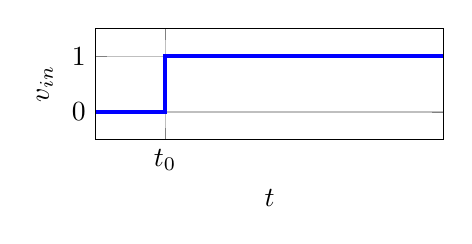
\begin{tikzpicture}
            \begin{axis}[
                width=6cm, height=3cm,
                xlabel={$t$},
                ylabel={$v_{in}$},
                domain=0:5,
                samples=100,
                grid=major,
                xmin=0, xmax=5,
                ymin=-0.5, ymax=1.5,
                ytick={0,1},
                xtick={1},
                xticklabels={$t_0$},
            ]
            \addplot[blue, very thick, const plot] coordinates {(0,0) (1,0) (1,1) (5,1)};
            \end{axis}
        \end{tikzpicture}
        \end{figure}
        
        \begin{figure}[htb]
        \centering
        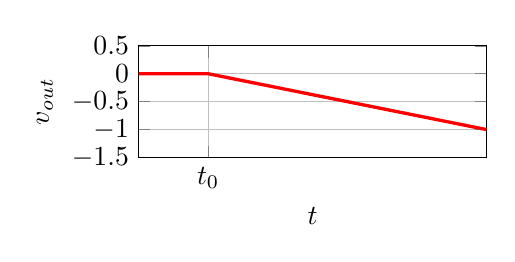
\begin{tikzpicture}
            \begin{axis}[
                width=6cm, height=3cm,
                xlabel={$t$},
                ylabel={$v_{out}$},
                domain=0:5,
                samples=100,
                grid=major,
                xmin=0, xmax=5,
                ymin=-1.5, ymax=0.5,
                xtick={1},
                xticklabels={$t_0$},
            ]
            \addplot[red, very thick] coordinates {(0,0) (1,0) (5,-1)};
            \end{axis}
        \end{tikzpicture}
        \caption{Step input produces ramp output}
        \end{figure}
        
    \column{0.48\textwidth}
        \textbf{Example 2: Square Wave Input}
        
        \begin{figure}[htb]
        \centering
        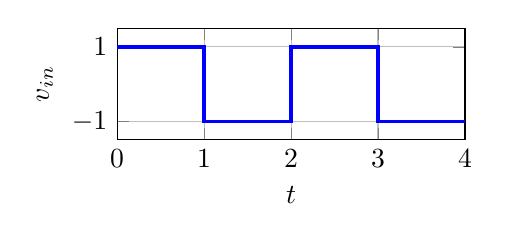
\begin{tikzpicture}
            \begin{axis}[
                width=6cm, height=3cm,
                xlabel={$t$},
                ylabel={$v_{in}$},
                domain=0:4,
                samples=100,
                grid=major,
                xmin=0, xmax=4,
                ymin=-1.5, ymax=1.5,
                ytick={-1,1},
            ]
            \addplot[blue, very thick, const plot] coordinates {
                (0,1) (1,1) (1,-1) (2,-1) (2,1) (3,1) (3,-1) (4,-1)
            };
            \end{axis}
        \end{tikzpicture}
        \end{figure}
        
        \begin{figure}[htb]
        \centering
        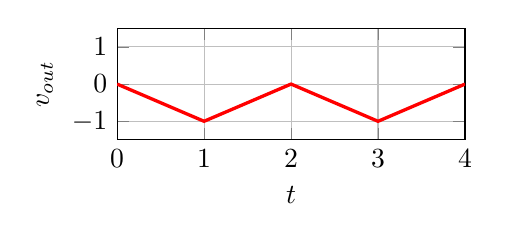
\begin{tikzpicture}
            \begin{axis}[
                width=6cm, height=3cm,
                xlabel={$t$},
                ylabel={$v_{out}$},
                domain=0:4,
                samples=100,
                grid=major,
                xmin=0, xmax=4,
                ymin=-1.5, ymax=1.5,
            ]
            \addplot[red, very thick] coordinates {
                (0,0) (1,-1) (2,0) (3,-1) (4,0)
            };
            \end{axis}
        \end{tikzpicture}
        \caption{Square wave produces triangle wave}
        \end{figure}
        
    \end{columns}
    
\end{frame}

\section{Differentiator}

\begin{frame}{The Differentiator}
    
    \begin{columns}[t]
    \column{0.48\textwidth}
        \textbf{Circuit Configuration}:
        
        \begin{figure}[htb]
        \centering
        \begin{circuitikz}[scale=1.0]
            % Input through capacitor
            \draw (0,0) to[C, l=$C$, o-] (2,0);
            
            % Op-amp
            \draw (3,-0.5) node[op amp, yscale=1.3] (opamp) {};
            \draw (2,0) |- (opamp.-);
            
            % Ground to noninverting
            \draw (opamp.+) -- ++(0,-0.5) node[ground] {};
            
            % Feedback resistor
            \draw (opamp.-) -- ++(0,1.5) coordinate(fb1);
            \draw (fb1) to[R, l=$R$] (fb1 -| opamp.out);
            \draw (opamp.out) |- (fb1 -| opamp.out);
            
            % Output
            \draw (opamp.out) to[short, -o] (5.5,-0.5) node[right] {$v_{out}$};
            
            % Labels
            \node[left] at (0,0) {$v_{in}$};
            \node at (2,0) [above] {$v_-=0$};
            
        \end{circuitikz}
        \caption{Inverting differentiator}
        \end{figure}
        
        \textbf{Note}:  Integrator with $R$ and $C$ swapped!
        
    \column{0.48\textwidth}
        \textbf{Analysis}:
        
        1. Virtual ground: $v_- = 0$
        
        2. Capacitor current:
        \[
        i_C = C \frac{dv_C}{dt} = C \frac{d(v_{in} - 0)}{dt}
        \]
        \[
        i_C = C \frac{dv_{in}}{dt}
        \]
        
        3. Since $i_- = 0$, $i_C$ flows through $R$:
        \[
        i_R = i_C = C \frac{dv_{in}}{dt}
        \]
        
        4. Output voltage:
        \[
        v_{out} = 0 - i_R R = -RC \frac{dv_{in}}{dt}
        \]
        
        \[
        \boxed{v_{out}(t) = -RC \frac{dv_{in}}{dt}}
        \]
        
    \end{columns}
    
\end{frame}

\begin{frame}{Differentiator:  Characteristics and Issues}
    
    \begin{columns}[t]
    \column{0.48\textwidth}
        \textbf{Transfer Function}:
        
        Time domain:
        \[
        v_{out} = -RC \frac{dv_{in}}{dt}
        \]
        
        Frequency domain: 
        \[
        \boxed{\frac{V_{out}(j\omega)}{V_{in}(j\omega)} = -j\omega RC}
        \]
        
        Magnitude:
        \[
        \left|H(j\omega)\right| = \omega RC
        \]
        
        \begin{itemize}
            \item Gain increases with frequency
            \item +20 dB/decade slope
            \item Amplifies high-frequency noise! 
        \end{itemize}
        
    \column{0.48\textwidth}
        \textbf{Practical Problems}:
        
        \begin{enumerate}
            \item \textbf{Noise amplification}
            \begin{itemize}
                \item High-frequency noise magnified
                \item Can saturate output
            \end{itemize}
            
            \item \textbf{Stability issues}
            \begin{itemize}
                \item Phase shift can cause oscillation
                \item Needs compensation
            \end{itemize}
        \end{enumerate}
        
        \vspace{0.3cm}
        
        \textbf{Practical Solution}:
        
        Add small resistor $R_s$ in series with $C$:
        \begin{itemize}
            \item Limits high-frequency gain
            \item Improves stability
            \item $R_s \ll R$ (typically $R_s \approx R/10$)
        \end{itemize}
        
        \vspace{0.3cm}
        
        \begin{alertblock}{Warning}
            Differentiators are rarely used in practice due to noise sensitivity
        \end{alertblock}
        
    \end{columns}
    
\end{frame}

\begin{frame}{Differentiator:  Waveform Examples}
    
    \begin{columns}[t]
    \column{0.48\textwidth}
        \textbf{Example 1: Ramp Input}
        
        \begin{figure}[htb]
        \centering
        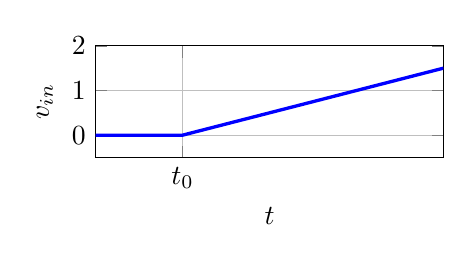
\begin{tikzpicture}
            \begin{axis}[
                width=6cm, height=3cm,
                xlabel={$t$},
                ylabel={$v_{in}$},
                domain=0:4,
                samples=100,
                grid=major,
                xmin=0, xmax=4,
                ymin=-0.5, ymax=2,
                xtick={1},
                xticklabels={$t_0$},
            ]
            \addplot[blue, very thick] coordinates {(0,0) (1,0) (4,1.5)};
            \end{axis}
        \end{tikzpicture}
        \end{figure}
        
        \begin{figure}[htb]
        \centering
        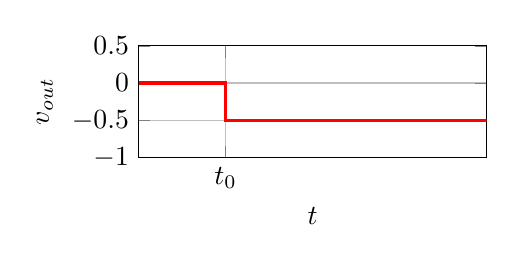
\begin{tikzpicture}
            \begin{axis}[
                width=6cm, height=3cm,
                xlabel={$t$},
                ylabel={$v_{out}$},
                domain=0:4,
                samples=100,
                grid=major,
                xmin=0, xmax=4,
                ymin=-1, ymax=0.5,
                xtick={1},
                xticklabels={$t_0$},
            ]
            \addplot[red, very thick, const plot] coordinates {(0,0) (1,0) (1,-0.5) (4,-0.5)};
            \end{axis}
        \end{tikzpicture}
        \caption{Ramp input produces constant output}
        \end{figure}
        
    \column{0.48\textwidth}
        \textbf{Example 2: Triangle Wave Input}
        
        \begin{figure}[htb]
        \centering
        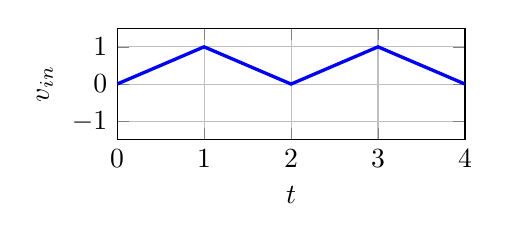
\begin{tikzpicture}
            \begin{axis}[
                width=6cm, height=3cm,
                xlabel={$t$},
                ylabel={$v_{in}$},
                domain=0:4,
                samples=100,
                grid=major,
                xmin=0, xmax=4,
                ymin=-1.5, ymax=1.5,
            ]
            \addplot[blue, very thick] coordinates {
                (0,0) (1,1) (2,0) (3,1) (4,0)
            };
            \end{axis}
        \end{tikzpicture}
        \end{figure}
        
        \begin{figure}[htb]
        \centering
        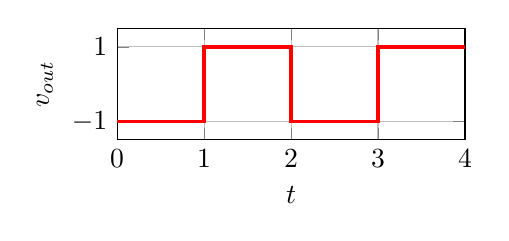
\begin{tikzpicture}
            \begin{axis}[
                width=6cm, height=3cm,
                xlabel={$t$},
                ylabel={$v_{out}$},
                domain=0:4,
                samples=100,
                grid=major,
                xmin=0, xmax=4,
                ymin=-1.5, ymax=1.5,
                ytick={-1,1},
            ]
            \addplot[red, very thick, const plot] coordinates {
                (0,-1) (1,-1) (1,1) (2,1) (2,-1) (3,-1) (3,1) (4,1)
            };
            \end{axis}
        \end{tikzpicture}
        \caption{Triangle wave produces square wave}
        \end{figure}
        
    \end{columns}
    
\end{frame}

\section{Summary and Practice}

\begin{frame}{Summary:  Op-Amp Applications}
    
    \begin{table}
    \centering
    \small
    \begin{tabular}{|l|c|c|l|}
    \hline
    \textbf{Configuration} & \textbf{Gain} & \textbf{$R_{in}$} & \textbf{Application} \\
    \hline
    Inverting & $-\frac{R_f}{R_1}$ & $R_1$ & Amplification with inversion \\
    \hline
    Noninverting & $1 + \frac{R_f}{R_1}$ & $\infty$ & Amplification, no inversion \\
    \hline
    Voltage Follower & 1 & $\infty$ & Buffering, impedance matching \\
    \hline
    Summing & $-\sum \frac{R_f}{R_i}v_i$ & $R_i$ & Audio mixing, DAC \\
    \hline
    Difference & $\frac{R_2}{R_1}(v_2-v_1)$ & finite & Instrumentation \\
    \hline
    Integrator & $-\frac{1}{RC}\int v_{in} dt$ & $\infty$ (AC) & Analog computation, filters \\
    \hline
    Differentiator & $-RC \frac{dv_{in}}{dt}$ & $\to 0$ (HF) & Rarely used (noise!) \\
    \hline
    \end{tabular}
    \caption{Summary of op-amp configurations}
    \end{table}
    
    \vspace{0.3cm}
    
    \begin{block}{Key Analysis Steps}
        \begin{enumerate}
            \item Identify configuration
            \item Apply virtual short:  $v_+ = v_-$ (with negative feedback)
            \item Apply zero input current:  $i_+ = i_- = 0$
            \item Use KCL at input nodes
            \item Solve for output voltage
        \end{enumerate}
    \end{block}
    
\end{frame}

\begin{frame}{Practice Problem 1}
    
    \textbf{Given}:  An inverting amplifier with $R_1 = 4.7$ k$\Omega$ and $R_f = 47$ k$\Omega$
    
    \vspace{0.3cm}
    
    \textbf{Find}:
    \begin{enumerate}[(a)]
        \item The voltage gain $A_v$
        \item The input impedance $R_{in}$
        \item If $v_{in} = 0.5$ V, what is $v_{out}$?
        \item What resistor value should $R_f$ be to achieve $A_v = -15$?
    \end{enumerate}
    
    \vspace{0.5cm}
    
    \textbf{Hint}: Use $A_v = -\frac{R_f}{R_1}$ and $R_{in} = R_1$
    
\end{frame}

\ifshowsolutions
\begin{frame}{Practice Problem 1 Solution}
    
    \textbf{Given}: $R_1 = 4.7$ k$\Omega$, $R_f = 47$ k$\Omega$
    
    \vspace{0.3cm}
    
    \textbf{Solutions}:
    
    (a) Voltage gain: 
    \[
    A_v = -\frac{R_f}{R_1} = -\frac{47\text{ k}\Omega}{4.7\text{ k}\Omega} = \boxed{-10 \text{ V/V}}
    \]
    
    (b) Input impedance:
    \[
    R_{in} = R_1 = \boxed{4.7 \text{ k}\Omega}
    \]
    
    (c) Output voltage: 
    \[
    v_{out} = A_v \cdot v_{in} = (-10)(0.5\text{ V}) = \boxed{-5 \text{ V}}
    \]
    
    (d) For $A_v = -15$: 
    \[
    -15 = -\frac{R_f}{4.7\text{ k}\Omega} \Rightarrow R_f = 15 \times 4.7\text{ k}\Omega = \boxed{70.5 \text{ k}\Omega}
    \]
    
    (Use standard value 68 k$\Omega$ or 75 k$\Omega$ in practice)
    
\end{frame}
\fi

\begin{frame}{Practice Problem 2}
    
    \textbf{Given}: A noninverting amplifier with the following requirements:
    \begin{itemize}
        \item Voltage gain:  $A_v = 5$
        \item Input voltage: $v_{in} = 0.2$ V
        \item Choose $R_1 = 10$ k$\Omega$
    \end{itemize}
    
    \vspace{0.3cm}
    
    \textbf{Find}: 
    \begin{enumerate}[(a)]
        \item The required value of $R_f$
        \item The output voltage $v_{out}$
        \item The input impedance
        \item If you need $A_v = 1$ (unity gain buffer), what should the circuit look like?
    \end{enumerate}
    
    \vspace{0.5cm}
    
    \textbf{Hint}: Use $A_v = 1 + \frac{R_f}{R_1}$
    
\end{frame}

\ifshowsolutions
\begin{frame}{Practice Problem 2 Solution}
    
    \textbf{Given}: $A_v = 5$, $R_1 = 10$ k$\Omega$, $v_{in} = 0.2$ V
    
    \vspace{0.3cm}
    
    \textbf{Solutions}:
    
    (a) Required $R_f$:
    \[
    5 = 1 + \frac{R_f}{10\text{ k}\Omega}
    \]
    \[
    \frac{R_f}{10\text{ k}\Omega} = 4 \Rightarrow R_f = \boxed{40 \text{ k}\Omega}
    \]
    
    (b) Output voltage:
    \[
    v_{out} = A_v \cdot v_{in} = 5 \times 0.2\text{ V} = \boxed{1.0 \text{ V}}
    \]
    
    (c) Input impedance:
    \[
    R_{in} = \boxed{\infty} \text{ (ideally)}
    \]
    
    (d) For unity gain buffer ($A_v = 1$):
    \begin{itemize}
        \item Connect output directly to inverting input (direct feedback)
        \item Remove $R_1$ and $R_f$
        \item Input to noninverting terminal
    \end{itemize}
    
\end{frame}
\fi

\begin{frame}{Practice Problem 3}
    
    \textbf{Given}: A summing amplifier with three inputs
    \begin{itemize}
        \item $R_1 = 10$ k$\Omega$, $R_2 = 20$ k$\Omega$, $R_3 = 5$ k$\Omega$
        \item $R_f = 20$ k$\Omega$
        \item Input voltages: $v_1 = 1$ V, $v_2 = 0.5$ V, $v_3 = -0.25$ V
    \end{itemize}
    
    \vspace{0.3cm}
    
    \textbf{Find}:
    \begin{enumerate}[(a)]
        \item The weight (coefficient) for each input
        \item The output voltage $v_{out}$
        \item If you want equal weights for all inputs, what should the resistor values be?
    \end{enumerate}
    
    \vspace{0.5cm}
    
    \textbf{Hint}: Use $v_{out} = -\left(\frac{R_f}{R_1}v_1 + \frac{R_f}{R_2}v_2 + \frac{R_f}{R_3}v_3\right)$
    
\end{frame}

\ifshowsolutions
\begin{frame}{Practice Problem 3 Solution}
    
    \textbf{Given}: $R_f = 20$ k$\Omega$, $R_1 = 10$ k$\Omega$, $R_2 = 20$ k$\Omega$, $R_3 = 5$ k$\Omega$
    
    \textbf{Inputs}:  $v_1 = 1$ V, $v_2 = 0.5$ V, $v_3 = -0.25$ V
    
    \vspace{0.3cm}
    
    \textbf{Solutions}:
    
    (a) Weights:
    \[
    w_1 = \frac{R_f}{R_1} = \frac{20}{10} = \boxed{2}
    \]
    \[
    w_2 = \frac{R_f}{R_2} = \frac{20}{20} = \boxed{1}
    \]
    \[
    w_3 = \frac{R_f}{R_3} = \frac{20}{5} = \boxed{4}
    \]
    
    (b) Output voltage:
    \[
    v_{out} = -(2 \times 1 + 1 \times 0.5 + 4 \times (-0.25))
    \]
    \[
    v_{out} = -(2 + 0.5 - 1) = \boxed{-1.5 \text{ V}}
    \]
    
    (c) For equal weights:  $R_1 = R_2 = R_3 = R$ (any equal value, e.g., 10 k$\Omega$)
    
\end{frame}
\fi

\begin{frame}{Practice Problem 4}
    
    \textbf{Given}: An integrator circuit with $R = 100$ k$\Omega$ and $C = 1$ $\mu$F
    
    \vspace{0.3cm}
    
    \textbf{Find}:
    \begin{enumerate}[(a)]
        \item The time constant $\tau = RC$
        \item If a constant input $v_{in} = 2$ V is applied starting at $t = 0$ (with $v_{out}(0) = 0$), find $v_{out}$ at $t = 0.1$ s
        \item At what time will the output reach $-5$ V?
        \item What is the magnitude of the transfer function at $f = 10$ Hz?
    \end{enumerate}
    
    \vspace{0.5cm}
    
    \textbf{Hint}: $v_{out}(t) = -\frac{1}{RC} \int_0^t v_{in}(\tau) d\tau$, and $|H(f)| = \frac{1}{2\pi f RC}$
    
\end{frame}

\ifshowsolutions
\begin{frame}{Practice Problem 4 Solution}
    
    \textbf{Given}: $R = 100$ k$\Omega$, $C = 1$ $\mu$F, $v_{in} = 2$ V (constant)
    
    \vspace{0.3cm}
    
    \textbf{Solutions}: 
    
    (a) Time constant:
    \[
    \tau = RC = (100 \times 10^3)(1 \times 10^{-6}) = \boxed{0.1 \text{ s}}
    \]
    
    (b) At $t = 0.1$ s:
    \[
    v_{out}(t) = -\frac{1}{RC} \int_0^t 2 \, d\tau = -\frac{2}{RC} \cdot t
    \]
    \[
    v_{out}(0.1) = -\frac{2}{0.1} \times 0.1 = \boxed{-2 \text{ V}}
    \]
    
    (c) For $v_{out} = -5$ V:
    \[
    -5 = -\frac{2}{0.1} \cdot t \Rightarrow t = \frac{5 \times 0.1}{2} = \boxed{0.25 \text{ s}}
    \]
    
    (d) At $f = 10$ Hz: 
    \[
    |H(f)| = \frac{1}{2\pi f RC} = \frac{1}{2\pi (10)(0.1)} = \frac{1}{2\pi} \approx \boxed{0.159}
    \]
    
\end{frame}
\fi

\begin{frame}{Practice Problem 5}
    
    \textbf{Given}: A difference amplifier with the following components:
    \begin{itemize}
        \item $R_1 = R_3 = 10$ k$\Omega$
        \item $R_2 = R_4 = 50$ k$\Omega$
        \item Input voltages: $v_1 = 2. 5$ V, $v_2 = 3.0$ V
    \end{itemize}
    
    \vspace{0.3cm}
    
    \textbf{Find}: 
    \begin{enumerate}[(a)]
        \item Verify that the resistor matching condition is satisfied
        \item The differential gain $A_d$
        \item The output voltage $v_{out}$
        \item If $v_1 = v_2 = 2.5$ V (common-mode), what is $v_{out}$ (ideally)?
    \end{enumerate}
    
    \vspace{0.5cm}
    
    \textbf{Hint}:  Matching condition: $\frac{R_2}{R_1} = \frac{R_4}{R_3}$, and $v_{out} = A_d(v_2 - v_1)$
    
\end{frame}

\ifshowsolutions
\begin{frame}{Practice Problem 5 Solution}
    
    \textbf{Given}: $R_1 = R_3 = 10$ k$\Omega$, $R_2 = R_4 = 50$ k$\Omega$
    
    \textbf{Inputs}:  $v_1 = 2.5$ V, $v_2 = 3.0$ V
    
    \vspace{0.3cm}
    
    \textbf{Solutions}:
    
    (a) Check matching condition:
    \[
    \frac{R_2}{R_1} = \frac{50}{10} = 5, \quad \frac{R_4}{R_3} = \frac{50}{10} = 5
    \]
    \[
    \boxed{\frac{R_2}{R_1} = \frac{R_4}{R_3} \checkmark} \text{ (condition satisfied)}
    \]
    
    (b) Differential gain:
    \[
    A_d = \frac{R_2}{R_1} = \frac{50}{10} = \boxed{5}
    \]
    
    (c) Output voltage:
    \[
    v_{out} = A_d(v_2 - v_1) = 5(3.0 - 2.5) = 5(0.5) = \boxed{2.5 \text{ V}}
    \]
    
    (d) Common-mode input ($v_1 = v_2$):
    \[
    v_{out} = A_d(v_2 - v_1) = 5(2.5 - 2.5) = \boxed{0 \text{ V}}
    \]
    (Perfect rejection with ideal op-amp and matched resistors)
    
\end{frame}
\fi

\begin{frame}{Advanced Application: Instrumentation Amplifier (Preview)}
    
    \begin{columns}[t]
    \column{0.48\textwidth}
        \textbf{Limitations of Simple Difference Amp}:
        \begin{itemize}
            \item Finite input impedance
            \item Limited CMRR (requires precise matching)
            \item Gain-impedance tradeoff
        \end{itemize}
        
        \vspace{0.3cm}
        
        \textbf{Instrumentation Amplifier}:
        \begin{itemize}
            \item Three op-amp configuration
            \item Very high input impedance (both inputs)
            \item Excellent CMRR (>100 dB)
            \item Single resistor sets gain
            \item Industry standard for precision measurement
        \end{itemize}
        
    \column{0.48\textwidth}
        \begin{figure}[htb]
        \centering
        \begin{circuitikz}[scale=0.65]
            % First stage - two op-amps
            \draw (0,2) node[op amp, yscale=0.8] (opamp1) {};
            \draw (0,-1) node[op amp, yscale=0.8, xscale=-1] (opamp2) {};
            
            % Inputs
            \draw (opamp1.+) -- ++(-0.5,0) to[short, -o] ++(-0.3,0) node[left] {$v_1$};
            \draw (opamp2.-) -- ++(-0.5,0) to[short, -o] ++(-0.3,0) node[left] {$v_2$};
            
            % Gain resistor between inverting inputs
            \draw (opamp1.-) to[R, l=$R_G$] (opamp2.+);
            
            % Feedback resistors
            \draw (opamp1.-) -- ++(0,0.8) to[R, l=$R$] ++(1. 5,0) -| (opamp1.out);
            \draw (opamp2.+) -- ++(0,-0.8) to[R, l_=$R$] ++(1.5,0) -| (opamp2.out);
            
            % Second stage - difference amplifier
            \draw (4,0. 5) node[op amp] (opamp3) {};
            
            % Connections to difference amp
            \draw (opamp1.out) to[R, l=$R$] (opamp3.-);
            \draw (opamp2.out) to[R, l=$R$] (opamp3.+);
            \draw (opamp3.+) to[R, l_=$R$] ++(0,-1. 5) node[ground] {};
            \draw (opamp3.-) -- ++(0,1) to[R, l=$R$] ++(1.5,0) -| (opamp3.out);
            
            % Output
            \draw (opamp3.out) to[short, -o] ++(0.5,0) node[right] {$v_{out}$};
            
        \end{circuitikz}
        \caption{Three op-amp instrumentation amplifier}
        \end{figure}
        
        \[
        A_v = \left(1 + \frac{2R}{R_G}\right)
        \]
        
    \end{columns}
    
    \begin{block}{Note}
        We'll study this in more detail when we cover precision amplifiers
    \end{block}
    
\end{frame}

\begin{frame}{Comparison of Configurations}
    
    \begin{table}
    \centering
    \small
    \begin{tabular}{|l|c|c|c|}
    \hline
    \textbf{Feature} & \textbf{Inverting} & \textbf{Noninverting} & \textbf{Difference} \\
    \hline
    Phase shift & 180° & 0° & 0° (for $v_2-v_1$) \\
    \hline
    Input impedance & $R_1$ & $\infty$ & Finite at both \\
    \hline
    Minimum gain & 0 (can attenuate) & 1 & 0 \\
    \hline
    Gain polarity & Negative & Positive & Positive \\
    \hline
    Complexity & Simple & Simple & Moderate \\
    \hline
    Virtual ground & Yes (at $v_-$) & No & No \\
    \hline
    CMRR & N/A & N/A & Depends on matching \\
    \hline
    \end{tabular}
    \caption{Comparison of basic op-amp configurations}
    \end{table}
    
    \vspace{0.3cm}
    
    \begin{block}{Design Guidelines}
        \begin{itemize}
            \item Use \textbf{inverting} when:  phase inversion acceptable, moderate $R_{in}$ OK
            \item Use \textbf{noninverting} when: high $R_{in}$ needed, no phase inversion
            \item Use \textbf{difference} when: differential measurement needed, CMRR important
            \item Use \textbf{integrator} for: low-pass filtering, waveform generation
            \item \textbf{Avoid differentiator} unless absolutely necessary (noise!)
        \end{itemize}
    \end{block}
    
\end{frame}

\begin{frame}{Practical Considerations}
    
    \begin{columns}[t]
    \column{0.48\textwidth}
        \textbf{Resistor Selection}:
        \begin{itemize}
            \item Typical range: 1 k$\Omega$ to 1 M$\Omega$
            \item Too low: excessive current, power
            \item Too high: noise pickup, offset errors
            \item Use 1\% or better for precision
            \item Match resistors for difference amp
        \end{itemize}
        
        \vspace{0.3cm}
        
        \textbf{Capacitor Selection}:
        \begin{itemize}
            \item Integrator:  low-leakage (polypropylene, polyester)
            \item Avoid electrolytic for precision
            \item Consider temperature coefficients
            \item ESR affects high-frequency performance
        \end{itemize}
        
    \column{0.48\textwidth}
        \textbf{Common Mistakes}:
        \begin{enumerate}
            \item Forgetting DC path (integrator saturation)
            \item Exceeding op-amp output current limit
            \item Ignoring bandwidth limitations
            \item Poor layout causing oscillations
            \item Wrong polarity on electrolytic caps
        \end{enumerate}
        
        \vspace{0.3cm}
        
        \textbf{Verification Steps}:
        \begin{itemize}
            \item Check DC operating point
            \item Verify gain with known input
            \item Test frequency response
            \item Check for distortion/clipping
            \item Measure with realistic loads
        \end{itemize}
        
    \end{columns}
    
\end{frame}




\end{document}